\begin{pastexam}[label={px:ntust-115-ice-10}]{臺科大資工所 115 學年度 第 II-2 題}
（填充）

(5\%) Consider the binary tree shown in the Fig.~1. Let $a$ be the 5-th element of the inorder traversal, and
let $b$ be the 8-th element of the preorder traversal. The value of $a-b$ is \blank{B}.

\begin{center}
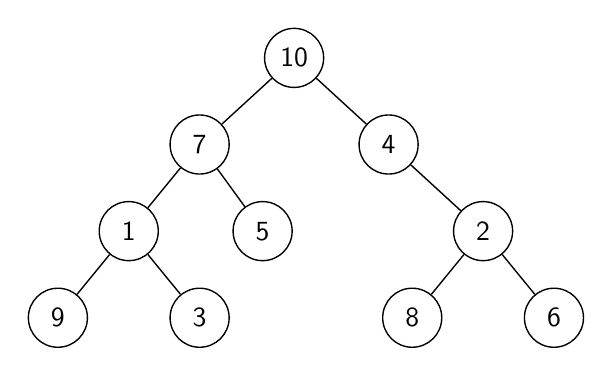
\begin{tikzpicture}[x=1cm,y=-1cm,
  every node/.style={circle,draw,line width=0.5pt,minimum size=7.5mm,inner sep=0pt,font=\sffamily}]
\node (n10) at (0,0) {10};
\node (n7) at (-1.2,1.1) {7};
\node (n4) at (1.2,1.1) {4};
\node (n1) at (-2.1,2.2) {1};
\node (n5) at (-0.4,2.2) {5};
\node (n2) at (2.4,2.2) {2};
\node (n9) at (-3,3.3) {9};
\node (n3) at (-1.2,3.3) {3};
\node (n8) at (1.5,3.3) {8};
\node (n6) at (3.3,3.3) {6};
\draw[line width=0.5pt] (n10)--(n7) (n10)--(n4) (n7)--(n1) (n7)--(n5) (n4)--(n2)
  (n1)--(n9) (n1)--(n3) (n2)--(n8) (n2)--(n6);
\end{tikzpicture}

Fig.~1 A given binary tree
\end{center}
\end{pastexam}

\begin{pastsoln}
答案：(B) $= 3$。

先讀出樹：根 $10$，左孩子 $7$、右孩子 $4$；$7$ 的孩子是 $1$（左）、$5$（右）；$1$ 的孩子是 $9$、$3$；$4$ 只有
\textbf{右}孩子 $2$；$2$ 的孩子是 $8$、$6$。

\textbf{中序}（左、根、右，資結書虛擬碼~7.1）：
\begin{itemize}
\item 左子樹 $7$：先走 $1$ 的子樹得 $9, 1, 3$，再 $7$，再 $5$：$9, 1, 3, 7, 5$。
\item 根 $10$。
\item 右子樹 $4$：$4$ 沒有左子樹，先印 $4$，再走 $2$ 的子樹 $8, 2, 6$：$4, 8, 2, 6$。
\end{itemize}
中序是 $9, 1, 3, 7, \mathbf{5}, 10, 4, 8, 2, 6$，第 $5$ 個 $a = 5$。

\textbf{前序}（根、左、右）：先 $10$，再左子樹 $7, 1, 9, 3, 5$，最後右子樹 $4, 2, 8, 6$。 前序是
$10, 7, 1, 9, 3, 5, 4, \mathbf{2}, 8, 6$，第 $8$ 個 $b = 2$。

所以 $a - b = 5 - 2 = 3$。
\end{pastsoln}
